\graphicspath{{cpeg2/}}


\chapter{Robust Entry Guidance with Atmospheric Adaptation}
\label{sec:cpeg2}

Robust atmospheric entry guidance for blunt-body entry vehicles with bank angle modulation is achieved by combining online atmospheric density estimation with an updated version of the Convex Predictor-corrector Entry Guidance (CPEG) algorithm. During atmospheric entry, a square-root Extended Kalman Filter is used to estimate a ratio between the density of the experienced atmosphere with that of an approximate model, which is spline-fit based on MarsGRAM perturbed data. The information from this filter is used to modify the approximate model used by the guidance algorithm. The proposed update to CPEG includes time as a decision variable, dramatically improving the robustness of the algorithm. CPEG predicts the trajectory at each control call with a nonlinear simulation followed by a single convex trajectory optimization problem that updates the commanded bank angle derivative. The robustness and performance of this estimator and controller guidance architecture are demonstrated on a wide range of realistic Martian atmospheres and is able to achieve state-of-the-art accuracy with respect to altitude-triggered parachute deployment.

The contents of this chapter have been previously published at IEEE Aerospace Conference 2021 in \citet{tracy2023}


\section{Introduction}
Entry into the Martian atmosphere refers to the phase of Entry, Descent, and Landing (EDL) that occurs between the point at which the hypersonic entry vehicle first interfaces with the planet’s sensible atmosphere and the point at which the supersonic parachute is deployed. It is during this portion of the EDL that the vehicle is subjected to the most demanding flight conditions, during which both peak acceleration and peak heating are experienced \cite{way2007}. Large uncertainties in models of the Martian atmospheric environment make entry guidance challenging, and significantly degrade landing accuracy, where the landing accuracy is the distance between the landing target site and the actual landing site. Actual atmospheric density can deviate from predictions by a factor of two or more \cite{justh2013}, requiring guidance laws to combat uncertainty with frequent re-planning and reliance on conservative initial entry conditions. These approaches ultimately reduce performance and limit the potential landing sites that can be accessed on Mars \cite{li2014}. To enable precision landing, which could potentially increase the number of reachable sites of high scientific interest, we propose a new approach to entry guidance that can strategically account for and reduce the atmospheric model uncertainty during guided entry.
\begin{figure}[h!]
\centering
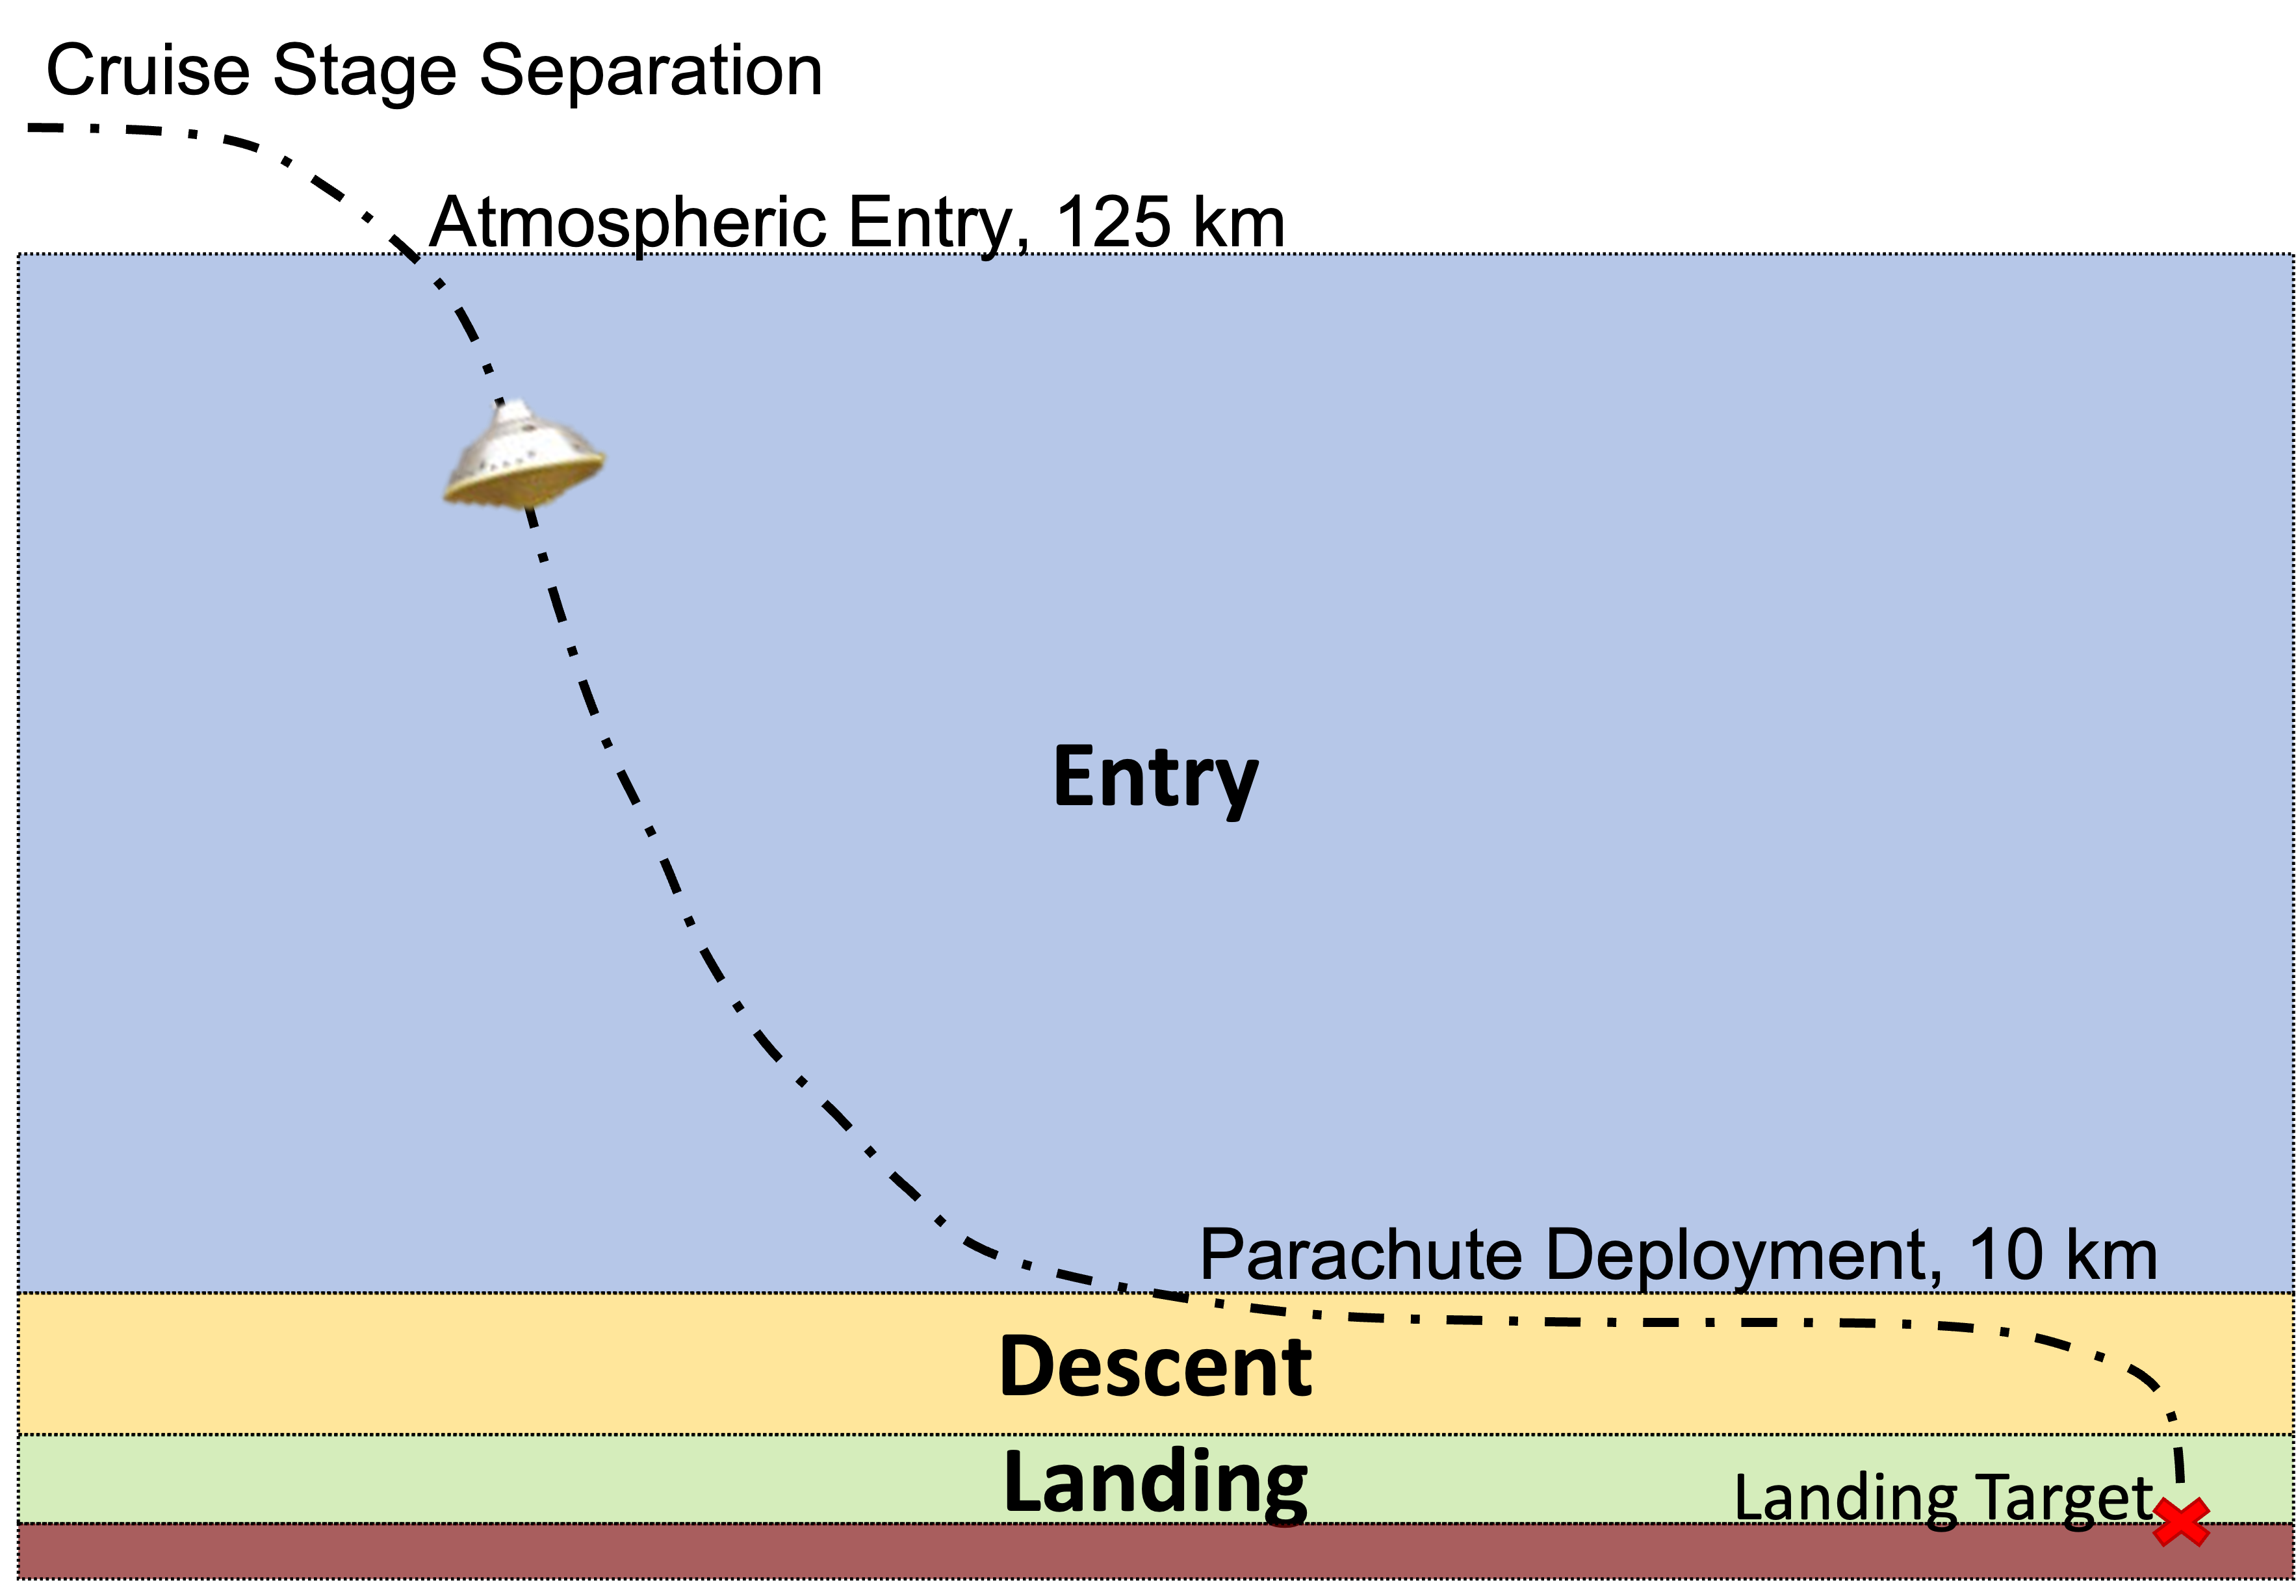
\includegraphics[width=0.5\linewidth]{entry.png}
  \caption{Cartoon representation of entry, descent, and landing.}
  \label{fig:entry}
\end{figure}

In the last few decades, predictor-corrector guidance algorithms have become the state-of-the-art; these have offered steadily improving landing accuracy with modest computational costs. These methods, like PredGuid \cite{putnam2010,putnam2014} and FNPEG \cite{lu2014a}, predict the trajectory of the entry vehicle with a nonlinear simulation, then use derivative or ``sensitivity'' information from the simulation to improve or ``correct'' the control plan \cite{lu2008,brunner2008}. This predictor-corrector framework offers improved landing accuracy compared to Apollo-era entry guidance methods \cite{brunner2012a} while being relatively simple to implement with low computational complexity. However, a significant drawback of traditional predictor-corrector guidance methods is their inability to generate complex control policies; many such methods are restricted to solving for a static bank angle, which means that the initial bank angle control profile predicted for the whole entry phase is considered constant; however, only during the prediction and correction phase, the guidance uses independent downrange and crossrange control to determine when the sign of the bank angle should flip. This simplicity severely limits the sophistication of the guidance method, and the resulting performance can chatter with multiple aggressive bank angle switches. Another limitation of existing predictor-corrector guidance strategies is their inability to incorporate real-time information about the Martian atmosphere, which is the largest source of uncertainty in the vehicle's dynamics, for prediction and correction purposes. 

Recently, there has been a growing interest in trajectory optimization methods for open-loop entry guidance for both Earth and Mars. This approach, in which the guidance problem is formulated as a numerical optimization problem, enables algorithms that can reason about the dynamics of the vehicle and constraints like actuator limits, state bounds, and heating limits. These optimization problems can be solved by a variety of numerical methods. As an example, sequential convex programming, in which a non-convex optimization problem is iteratively convexified and solved until convergence, has recently become popular \cite{wang2016,wang2018,mao2019,szmuk2019,szmuk2020,malyuta2021}. Alternatively, the trajectory optimization problem can be converted into a nonlinear program \cite{betts2001} and solved by a variety of off-the-shelf solvers, like SNOPT \cite{gill2005} or Ipopt \cite{wachter2006}, or by a more specialized trajectory optimization solver like ALTRO \cite{howell2019, jackson2021b}. While these trajectory optimization guidance methods offer more sophisticated and performant control plans than classical predictor-corrector methods, they can be prohibitively complex to implement on resource-constrained flight computers, and are still unable to account for real-time information about the atmosphere. 

A middle ground between simple predictor-corrector guidance schemes and offline trajectory optimization is the Convex Predictor-corrector Entry Guidance algorithm (CPEG) \cite{tracy2022a}. This method uses the same predictor-corrector framework as existing methods, but instead of solving for a simple static bank angle, it forms a convex trajectory optimization problem that solves for the correction to the nominal control plan. This approach enables the direct inclusion of any actuator or safety constraints and the ability to reason about complex control policies and the dynamics of the vehicle over the whole trajectory. By forming the convex trajectory optimization problem with a dynamics model linearized about the prediction rollout, the problem is guaranteed to always be feasible, and the convexity of the problem guarantees that an optimal solution can be computed in polynomial time \cite{boyd2004}. 

This work proposes an improvement to the CPEG algorithm that includes time as an optimization variable, allowing for the generation of trajectories with a free final time. This modification allows for significantly more flexibility when handling scenarios with multiple potentially successful control policies, since many trajectories can all be expressed using the same number of optimization variables. The absence of this feature in the original CPEG algorithm resulted in a lack of robustness when run online with significant model uncertainty. Additionally, this work directly addresses the main source of the uncertainty in the vehicle dynamics -- the atmospheric density -- by estimating information about the atmosphere online and including it in the approximate model used by CPEG. Our specific contributions include:
\begin{enumerate}
    \item A free-final-time extension of the Convex Predictor-corrector Entry Guidance algorithm
    \item An estimation architecture for atmospheric density and an atmospheric approximate model
    \item Validation of the combined controller and estimator on realistic density and wind dispersions from MarsGRAM \cite{justh2013}
\end{enumerate}

This paper proceeds by first describing the dynamics of the entry vehicle in Cartesian coordinates in Section \ref{sec:cpeg2:section3}, followed by the free-final-time version of CPEG in Section \ref{sec:cpeg2:section4}. The atmospheric density estimation approach is detailed in Section \ref{sec:cpeg2:section5}. Numerical experiments using Monte-Carlo sampling of atmospheric parameters from MarsGRAM are presented in Section \ref{sec:cpeg2:section6}. Finally, Section \ref{sec:cpeg2:section7} summarizes our conclusion.

\section{Entry Vehicle Dynamics}\label{sec:cpeg2:section3}
This work considers a blunt-body entry vehicle in the Martian atmosphere with the ability to modulate its bank angle $\sigma \in \R{}$. These entry vehicles are traditionally described and simulated in spherical coordinates using the “Vinh” model \cite{busemann1976,vinh1980,vinh2000,wang2018,wang2019a,lu2014a,gallais2007}. While this model is ubiquitous and well-studied, it suffers from numerical scaling issues due to the state vector including angles as well as distance and velocity, and is highly nonlinear in both the state and the control input. These shortcomings make optimization challenging and numerically unreliable. Alternatively, the state and dynamics of the entry vehicle can be equivalently described in a Mars-fixed Cartesian reference frame. This parametrization is more common in the powered-descent guidance literature \cite{blackmore2012, acikmese2007, acikmese2013}, and has much better numerical scaling, as well as linear kinematics, both of which make it a better fit for optimization-based control methods as detailed in \cite{tracy2022}. The dynamics of the entry vehicle with this state representation are the following:
\begin{align}
    \dot{r} &= v, \\ 
    \dot{v} &= a_L + a_D + a_g - 2 (\omega \times v) - \omega \times (\omega \times r).
\end{align}
% where $a_L \in \R{}$, $a_D \in \R{}$, and $a_g \in \R{}$ are, respectively, the accelerations due to lift, drag, and gravity, and $\omega \in \R{3}$ is the angular velocity of the planet in this Mars-fixed frame.  
The aerodynamic accelerations from lift and drag are dependent on the vehicle velocity relative to the atmosphere, including wind. The wind vector $w$ is expressed in the Mars-fixed frame, and the relative velocity is simply $v_{rel} = v + w$. The magnitude of the lift and drag accelerations can then be computed as follows:
\begin{align}
    L &= \frac{1}{2m} \rho A C_L \|v_{rel}\|^2, \\ 
    D &= \frac{1}{2m} \rho A C_D \|v_{rel}\|^2.
\end{align}
% where $A \in \R{}$ is the cross-sectional area of the vehicle, $C_L \in \R{}$ and $C_D \in \R{}$ are the coefficients of lift and drag respectively, $m \in \R{}$ is the mass of the vehicle, and $\rho$ is the atmospheric density. 
The hypersonic coefficients, $C_L$ and $C_D$ have been evaluated through the Newtonian flow theory for a blunted body, specifically: 
\begin{align}
    C_A &= (1-\sin{\delta}^4)  \dfrac{r_{nose}^2}{r_{base}^2} + (2\sin{\delta}^2 \cos{\alpha}^2 + \cos{\delta}^2 \sin{\alpha}^2)\left(1-\dfrac{r_{nose}^2}{r_{base}^2} \cos{\delta}^2\right),\\
    C_N &= \left(1-\dfrac{r_{nose}^2}{r_{base}^2} \cos{\delta}^2\right)\cos{\delta}^2\sin{2\alpha},\\
    C_L &= C_N\cos{\alpha}-C_A\sin{\alpha},\\
    C_D &= C_A\cos{\alpha}+C_N\sin{\alpha},
\end{align}
where $C_A$ is the axial force coefficient, $C_N$ is the normal force coefficient, $\delta$ is the cone angle of the blunted-cone vehicle,  $\alpha$ is the angle of attack, $r_{base}$ is the base radius, $r_{nose}$ is the nose radius of the hypersonic vehicle.
        
The direction of the drag acceleration is in the opposite direction of the relative velocity, expressed as:
\begin{align}
    a_D &= -D \frac{v_{rel}}{\|v_{rel}\|}.
\end{align}
The lift acceleration is directed using the bank angle $\sigma$, and is modeled and represented with two basis vectors $\hat{e}_1 \in \R{3}$ and $\hat{e}_2 \in \R{3}$, where together they span the plane orthogonal to the relative velocity of the vehicle in the atmosphere. These aerodynamic basis vectors are constructed as the following:
\begin{align}
    \hat{e}_1 &=  \frac{r \times v_{rel}}{\|r \times v_{rel}\|}, \\ 
    \hat{e}_2 &= \frac{v_{rel} \times \hat{e}_1}{\| v_{rel} \times \hat{e}_1 \|} .
\end{align}
Using these basis vectors, the lift acceleration can be computed as the following:
\begin{align}
    a_L &= L(\sin(\sigma) \hat{e}_1 + \cos(\sigma)\hat{e}_2).
\end{align}
The acceleration due to gravity can be calculated using any number of established methods ranging in fidelity from simple two-body gravity \cite{montenbruck2002}, to a more complex spherical harmonic expansion of the geopotential \cite{hirt2012,genova2016}. 

The largest amount of uncertainty in the dynamics of the entry vehicle comes from the atmosphere. Both the atmospheric density $\rho$, as well as the wind vector $w$ are highly uncertain. To visualize this uncertainty, Mars GRAM \cite{justh2013} was used to generate dispersions for these two parameters, which are shown in Fig. \ref{fig:mgdensity} and Fig. \ref{fig:mgwind}. A summary of the parameters used to run Mars GRAM is presented in Table \ref{tab:marsgram}. For the generation of atmospheric data points in highly perturbed environments, Mars GRAM not only uses random Monte Carlo samples that re-initialize the random number seed (NR1) for each sample but also has been set for different zoffsets, which are constant height offsets that modify the atmospheric density. Specifically, positive offsets increase density, while negative offsets decrease density. In addition, rpscale, the random perturbation scale was also set to the maximum, with increasing this factor intensifying the magnitude of the perturbation. The data have also been evaluated in the context of a global dust storm, through INTENS, which changes the dust storm intensity. 

\begin{table}[h!]
\centering
\caption{Mars GRAM nominal and dispersion parameters}
\begin{tabular}{cccc}
\hline \hline
Parameter & Value   & Parameter                                                                        & Value \\ \hline 
\begin{tabular}[c]{@{}c@{}}Initial Altitude, km\end{tabular} &
  125 &
  \begin{tabular}[c]{@{}c@{}}NR1\end{tabular} &
  {[}1,5001{]} \\
Date &
  6 August 2012 &
  \begin{tabular}[c]{@{}c@{}}zoffset, km\end{tabular} &
  \begin{tabular}[c]{@{}c@{}}Uniform Dist., {[}-3.25,3.25{]}\end{tabular} \\
Time      & 5:30:00 & \begin{tabular}[c]{@{}c@{}}rpscale\end{tabular} & 2     \\
\begin{tabular}[c]{@{}c@{}}Final Altitude, km\end{tabular} &
  10 &
  \begin{tabular}[c]{@{}c@{}}INTENS \end{tabular} &
  2\\
  \hline \hline
\end{tabular}
\label{tab:marsgram}
\end{table}

Since aerodynamic acceleration is the dominant term in the dynamics at the high speeds an entry vehicle experiences, the uncertainty in the atmospheric density results in a highly uncertain dynamics model. The uncertainty in the wind contributes to the model uncertainty, but less so than the density.  
\begin{figure}
    \centering
    \includegraphics{tikz/atmo_uncertainty/density_shaded.tikz}
    \caption{Dispersion of the atmospheric density as a function of altitude calculated with Mars GRAM.  The dynamics of the entry vehicle are heavily influenced by this density, and the dramatic uncertainty of this value motivates the need for more robust guidance schemes.}
    \label{fig:mgdensity}
\end{figure}
\begin{figure}
    \centering
    \includegraphics{tikz/atmo_uncertainty/wind_shaded.tikz}
    \caption{Dispersions of the east and north wind velocities in the Martian atmosphere as a function of altitude calculated with Mars GRAM. This range of atmospheric wind profiles is used in the Monte Carlo testing of the proposed entry guidance algorithm.}
    \label{fig:mgwind}
\end{figure}


\section{CPEG}\label{sec:cpeg2:section4}
Predictor-corrector guidance algorithms are a simple and effective way to control underactuated systems like the entry vehicle. These methods all share a general framework in which a nominal control policy is used to simulate a predicted trajectory, then a correction is made to the nominal control policy based on this prediction. Predictor-corrector methods have been the state of the art for entry guidance of blunt-body vehicles, but they are not without their shortcomings. Existing methods like FNPEG are only able to reason about simple static bank angle policies, and rely on independent crossrange and downrange logic to modulate the bank angle \cite{lu2008}. Alternatively, offline trajectory optimization allows for more complex control policies and the direct inclusion of constraints, but is significantly more expensive than predictor-corrector methods. A trajectory optimization problem in its most general form is the following,
\newpage
\begin{mini}<b>
  {x_{1:N},u_{1:N-1}}{\ell_N(x_N)+ \sum _{k=1}^{N-1}\ell_k(x_k, u_k)}{}{}
  \addConstraint{x_{k+1}= f(x_k,u_k)}{}{\quad k = 1 \ldots N-1} \labelOP{nlp}%\tag{test}
  \addConstraint{g_k(x_k, u_k)\leq 0 }{}{\quad k = 1 \ldots N-1} 
   \addConstraint{u_{min}\leq u_k \leq u_{max} }{}{\quad k = 1 \ldots N-1}
  \addConstraint{x_{min}\leq x_k \leq x_{max} }{}{\quad k = 1 \ldots N}
  % \addConstraint{\Delta t_{min} }{\leq \Delta t_k \leq \Delta t_{max} }{\forall k}
  % \addConstraint{x_N}{=x_{goal}}{},
 \end{mini}
where $x$ is the state, $u$ is the control, $\ell$ is the cost function, $f(x,u)$ is the discrete dynamics function, and $g(x,u)$ is a general constraint function. Problem \eqref{nlp} can be solved with a multitude of available trajectory optimization solvers, but they are prohibitively complex to run on board the entry vehicle. 
\subsection{Baseline CPEG}
The Convex Predictor-corrector Entry Guidance (CPEG) algorithm, introduced in \cite{tracy2022}, seeks to find a middle ground between simple predictor-corrector guidance methods and offline trajectory optimization. This is achieved by adopting the predictor-corrector framework, but solving a convex trajectory optimization problem for the correction instead of a simple update to a static bank angle like in FNPEG. This approach allows CPEG to reason about sophisticated control trajectories as well as the dynamics of the vehicle throughout the entirety of the trajectory. The convex optimization problem that makes up the correction portion of the algorithm is guaranteed to be feasible, and its optimum can be solved for at real-time rates \cite{mattingley2012}. 

In order for problem \eqref{nlp} to be convex, the cost and constraint functions must be convex. This means that problems with nonlinear dynamics, like the entry vehicle, must be approximated. We linearize the discrete dynamics function $f(x,u)$ about the predicted trajectory $(\bar{x},\bar{u})$:
\begin{align}
    \bar{x}_{k+1} + \delta x_{k+1} \approx f(\bar{x}_k,\bar{u}_k) + A_k \delta x_k + B_k \delta u_k, \label{taylor_series}
\end{align}
where $A_k$ and $B_k$ are the following Jacobians,
\begin{align}
    A_k &= \frac{\partial f(x_k,u_k)}{\partial x_k} \bigg\rvert _{\bar{x}_k,\bar{u}_k}, \label{jacob1}\\
    B_k &= \frac{\partial f(x_k,u_k)}{\partial u_k}\bigg\rvert _{\bar{x}_k,\bar{u}_k}. \label{jacob2}
\end{align}
Since the prediction was dynamically feasible, and $\bar{x}_{k+1} = f(\bar{x}_k,\bar{u}_k)$, equation \eqref{taylor_series} is reduced to
\begin{align}
    \delta x_{k+1} \approx   A_k \delta x_k + B_k \delta u_k.
\end{align}
From here, the convex correction problem is posed as,
% \todo{can we force this to be all on the same page? let's wait to fix everything before this point and if the problem is still there, we force it (G)}
\begin{mini}<b>
  {\delta x_{1:N},\delta u_{1:N-1}}{\ell_N(\bar{x}_N + \delta x_N)+ \sum _{k=1}^{N-1}\ell_k(\bar{x}_k + \delta x_k, \bar{u}_k + \delta u_k) }{}{}
  \addConstraint{\delta x_{k+1}=  A_k \delta x_k + B_k \delta u_k}{}{\quad k = 1 \ldots N-1} \labelOP{cto}%\tag{test}
  \addConstraint{g_k(\bar{x}_k + \delta x_k, \bar{u}_k + \delta u_k)\leq 0}{}{\quad k = 1 \ldots N-1} 
  \addConstraint{u_{min}\leq u_k \leq u_{max} }{}{\quad k = 1 \ldots N-1}
  \addConstraint{x_{min}\leq x_k \leq x_{max} }{}{\quad k = 1 \ldots N}
  \addConstraint{\delta u_{min}\leq \delta u_k \leq \delta u_{max} }{}{\quad k = 1 \ldots N-1}
  \addConstraint{\delta x_{min}\leq \delta x_k \leq \delta x_{max} }{}{\quad k = 1 \ldots N,}
  % \addConstraint{x_N}{=x_{goal}}{},
 \end{mini}
 where the bounds on $\delta x$ and $\delta u$ serve as a customizable trust region that ensures the step direction stays within a region of the state space where the linearization is accurate \cite{nocedal2006}. Since the linearization is evaluated about the dynamically feasible predicted trajectory, this optimization problem is guaranteed to have a feasible solution of all zeros for $\delta x$ and $\delta u$, eliminating one of the largest vulnerabilities in real-time optimization-based control. 

The full baseline CPEG algorithm is shown in Algorithm \ref{alg:flight}, where an initial condition and nominal control policy are used to simulate the entry vehicle until parachute deployment (the prediction), a linearized model is evaluated about this predicted trajectory, and a convex trajectory optimization problem \eqref{cto} is solved for the correction. 
  \begin{algorithm} [H]
	\begin{algorithmic}[1]
		\caption{CPEG Algorithm}\label{alg:flight}
		\State \textbf{function} $\operatorname{CEPG}(x_0, U$  \Comment{nominal control plan}
		% \While{$\|\delta U\| > $ tolerance}
    		\State $\quad \Bar{X}, \Bar{U} = \text{simulate}(x_0,U)$ \Comment{predict trajectory}
    		\State $\quad A,B = \text{linearize}(\Bar{X}, \Bar{U})$ \Comment{linearize about prediction}
    		\State $\quad \delta X,\delta U = \text{cvx}(\Bar{X}, \Bar{U}, A, B)$ \Comment{solve for correction} 
    	    \State $\quad U \mathrel{+}= \delta U $ \Comment{correct control plan}
		% \EndWhile
		\State \textbf{return} $U$ \Comment{return updated control plan}
	\end{algorithmic}
\end{algorithm}
\subsection{Variable-Time CPEG}
 We now extend CPEG to handle free-final-time problems where time is a decision variable. In the baseline algorithm, the prediction is done with a fixed time step and the simulation simply terminates when a parachute deployment trigger is satisfied. This means that the corrected control policy can result in a subsequent prediction with a different number of time steps. This characteristic of the baseline algorithm results in decreased robustness when there are multiple cost-equivalent trajectories in the cost landscape. In this case, CPEG can chatter between two or more control policies that are of different lengths but have equal cost. 

 To address this issue, an updated version of CPEG is proposed in this work that treats time as an explicit optimization variable, allowing for the time of parachute deployment to effectively be decided by the optimization solver, instead of solely by the prediction step. This updated version of CPEG is significantly more robust to chattering. The free-final-time modification can be incorporated into the existing CPEG framework by simply including the time step for each knot point as a control input. The resulting state variable $x \in \R{7}$ and control variable $u \in \R{2}$ are the following:
\begin{align}
    x &= [r^T, v^T, \sigma]^T, \\ 
    u &= [\dot{\sigma}, \Delta t]^T,
\end{align}
where $\Delta t \in \R{}$ is the size of the time step. We use the following cost function:
\begin{align}
    J(x,u) &= \gamma \|r_N - r_\text{target}\|^2 + \sum_{k=1}^{N-1} \beta \dot{\sigma}_k^2  + (\Delta t_k - \Delta t_\text{target})^2 ,
\end{align}
where $\gamma \in \R{}_+$ and $\beta \in \mathbb{R}_+$ are positive cost weights, $r_\text{target} \in \R{3}$ is the target position, and $\Delta t_\text{target} \in \R{}_+$ is target time-step size. These weights should be tuned such that the largest penalty is applied to the terminal position accuracy, and a sufficient penalty exists on the time-step size to keep the time steps positive and reasonable.

Each control correction requires the solution of a convex Quadratic Program (QP), of which there are many fast and robust solution methods available. This work utilized a custom implementation of the primal-dual interior point solver detailed in \cite{mattingley2012} and \cite{vandenberghe}. At the start of the QP solver, the inequality constraints are temporarily omitted and the closed-form solution to the equality-constrained QP is checked for feasibility. In many cases, the inequality constraints are inactive at the optimum, and this approach is able to solve the QP at the cost of solving a single linear system. 
% \todo{FYI: I removed some references to ``global'' since we're only getting the global solution to a convex approximation of the real problem. I thought it was a little confusing.}
\section{Atmospheric Estimation}\label{sec:cpeg2:section5}
During atmospheric entry guidance, the largest source of uncertainty in the dynamics comes from the atmosphere. The density of the atmosphere is highly variable based on the time of the year, weather, dust conditions, temperature, and space weather. Mars GRAM \cite{justh2013} is the highest fidelity tool available for the simulation of the Martian atmosphere, and it was used to sample 5,000 potential atmospheric density profiles. 1,000 of these profiles are shown in Fig. \ref{fig:mgdensity}, where there is significant uncertainty at higher altitudes, with better certainty at lower altitudes, though still varying by $10-20\%$. Because of this uncertainty, open-loop control policies perform poorly. 

To manage this uncertainty, we propose a simple and effective method for estimating critical information about the atmospheric density online during the entry process. The density of the Martian atmosphere roughly follows an exponential law, such that the difference in density between the surface and 125 km altitude, which is considered in this study as the entry interface, spans several orders of magnitude. Because of this large variation in magnitude, estimating the density directly in a Kalman Filter is numerically challenging. Another possible approach to tackle atmospheric uncertainties would be to directly model the atmosphere as an exponential and estimate the surface density and scale height \cite{markley2014}, but this approach suffers from severe ill-conditioning because the exponential dramatically amplifies errors at higher altitudes \cite{heidrich2021,dutta2014}. 

In place of estimating some parametrized version of the atmospheric density profile from scratch, we use an approach similar to \cite{roelke2009} where a Kalman filter for estimating the ratio between the observed and nominal atmospheres:
\begin{align}
    k_\rho = \frac{\rho_\text{observed}}{\rho_\text{nominal}},
\end{align}
where $\rho_\text{nominal}$ is computed offline and stored. Estimating $k_\rho$ directly is better behaved numerically because the estimator is simply looking to modify an existing approximate density profile, and the estimated value will always be near 1, regardless of altitude. The state and control for this filter are the following:
\begin{align}
    x_\text{kf} &= [r^T, v^T, \sigma, k_\rho]^T, \\ 
    u_\text{kf} &= \dot{\sigma},
\end{align}
where the dynamics for this state representation are the same as in section \ref{sec:cpeg2:section3}, with the exception that $\rho = k_\rho \cdot \rho_\text{approximate}$. The measurement model is assumed to come directly from the navigation system, with additive Gaussian white noise. To estimate $k_\rho$ effectively in the presence of highly variable dynamic pressure, a Square-Root Extended Kalman Filter (SQEKF) is used that allows for twice the dynamic range of the standard Extended Kalman Filter (EKF) \cite{kaminski1971}. This increased range and numerical robustness help to manage the potentially ill-conditioned covariance matrices present during entry guidance. A simple version of an SQEKF is demonstrated in \cite{tracy2022f} that leverages a highly mature QR decomposition routine to handle a majority of the computation \cite{strang1968}.

The SQEKF takes a system of the following form:
\begin{align}
	x_{k+1} &= f(x_k,u_k) + w_k , \\ 
    y_k &= g(x_k) + v_k ,
\end{align}
where $f(x,u)$ is the discrete time dynamics function, $g(x)$ is the measurement function, and $w \sim \mathcal{N}(0,W)$ and $v \sim \mathcal{N}(0,V)$ are the process and sensor noise terms, respectively. The SQEKF is able to achieve better precision than the standard EKF by representing covariance matrices by their upper-triangular matrix square roots (Cholesky factors) \cite{simon2006,vandermerwe2001,bar-shalom2002}. %This allows for covariance matrices that are poorly scaled to be represented in a much more uniform way, since the square root makes the values greater than one smaller, and the values less than one larger.
Using this notation, the SQEKF algorithm from \cite{tracy2022f} is shown in Algorithm \ref{alg:mgn}, where $\Gamma_W$ and $\Gamma_V$ are the upper triangular Cholesky factorizations of $W$ and $V$, and the function $\operatorname{qr_r}$ returns the upper triangular $R$ factor from a QR decomposition \cite{strang1968,howell2019}. The mean of the estimate is $\mu_{t|t}$, and the covariance $\Sigma$ is represented with its matrix square root $F$ such that $F^TF = \Sigma$. The performance of this filter on a realistic atmosphere sample from Mars GRAM is shown in Fig. \ref{fig:krho}. 
\begin{algorithm} 
	\begin{algorithmic}[1]
		\caption{Square Root Extended Kalman Filter}\label{alg:mgn}
		\State \textbf{function}  sqkf($\mu_{t|t},F_{t|t},u_t,y_{t+1},\Gamma_W,\Gamma_V)$
		\State 
		% \State \quad \# predict step 
            \State \quad $A_t = \partial f / \partial x |_{\mu_{t|t},u_t}$ \Comment{dynamics Jacobian}
		\State \quad $\mu_{t+1|t} = f(\mu_{t|t},u_t) $ \Comment{state prediction}
		\State \quad $F_{t+1|t} = \operatorname{qr_r} ( F_{t|t} A_t^T , \Gamma_W)$ \Comment{covariance prediction}
		\State 
		% \State \quad \# innovation
  \State \quad $C_t = \partial g / \partial x |_{\mu_{t+1|t}}$ \Comment{measurement Jacobian}
        \State \quad $z = y_{t+1} - g(\mu_{t+1|t})$ \Comment{measurement innovation}
        \State \quad $G = \operatorname{qr_r}(F_{t+1|t} C_t^T, \Gamma_V)$ \Comment{innovation covariance}
        \State \quad $L = [G^{-1}(G^{-T} C_t) F_{t+1|t}^TF_{t+1|t}]^T$ \Comment{Kalman gain}
        \State 
        % \State \quad \# update step 
        \State \quad $\mu_{t+1|t+1} = \mu_{t+1|t} + Lz $ \Comment{state update}
        \State \quad $F_{t+1|t+1} = \operatorname{qr_r}(F_{t+1|t}(I-LC_t)^T, \Gamma_VL^T)$ \Comment{covariance update}
        \State 
        \State \quad \textbf{return}($\mu_{t+1|t+1}, F_{t+1|t+1}$)
	\end{algorithmic}
\end{algorithm}
\begin{figure}
    \centering
    \includegraphics{tikz_v2/krho.tikz}
    \caption{Results from the atmospheric density estimator during entry guidance where the ratio between the actual and nominal densities, $k_\rho$, is shown alongside the true value. There is large uncertainty in the higher altitudes where the atmosphere is very thin, and again at lower altitudes where the velocity of the vehicle is such that aerodynamic forces are not as dominant in the dynamics.}
    \label{fig:krho}
\end{figure}

\section{Numerical Experiments}\label{sec:cpeg2:section6}
To validate the combined controller and estimator architecture, 1,000 Monte Carlo runs were used to test the robustness and performance of the algorithms. Each Monte Carlo run consists of an atmospheric density and wind sampled from Mars GRAM, as shown in Fig. \ref{fig:mgdensity} and Fig. \ref{fig:mgwind}. An initial position dispersion with a standard deviation of 1 km and initial bank angle dispersion of 5 degrees was used to further disambiguate between runs. The initial conditions coincide with the Mars Sample Return (MSL) initial conditions; specifically, the initial position had a mean altitude of 125 km, with a flight path angle of -15.5 degrees and entry velocity of 5.85 km/s \cite{braun2006, way2007}. The target was 632 km down range and 7.9 km cross range, with a parachute deployment triggered at 10 km altitude. Furthermore, the hypersonic vehicle considered has the same characteristics of the MSL vehicle; specifically, the vehicle is a 70 degrees sphere-cone, nose radius equal to 1.125 m, a base radius equal to 2.25 m, and an entry mass of 2800 kg \cite{braun2006}.

The variable-time CPEG algorithm was run with a nominal time step size of 2 seconds until the length of the trajectory was less than 50 knot points, at which point the nominal time step was lowered to 0.1 seconds. This algorithm was run at 5 Hz with one convex correction solution at each time step, 94\% of which were solved in a single iteration of the QP solver. A trust region was used to keep the updated trajectory in an area of the state space where the linearized dynamics model is still accurate, with $|\delta \sigma | \leq 20 ^\circ$ and $|\delta \Delta t |\leq 0.1 $. The SQEKF was initialized at an altitude of 60 km, and the estimated $k_\rho$ value was used in the dynamics model in CPEG. The measurement model in the SQEKF assumed full state observations from the navigation system, with conservative measurement error standard deviations of 100 meters for the position, and 20 cm/s for the velocity. 
% \todo{track down this 20 cm/s velocity error ref}

All 1,000 Monte Carlo runs were successful in deploying the parachute within 1km of the target, with the trajectories shown in Fig. \ref{fig:dr_cr} and Fig. \ref{fig:dr_alt}. Depending on the specific atmosphere and initial perturbation, there were two families of trajectories that the entry vehicle traversed. The bank-angle profiles for these trajectories are shown in Fig. \ref{fig:bank_angle}. The terminal errors for these runs are shown in Fig. \ref{fig:term_err}, with each individual run shown as well as a $3\sigma$ ellipse. 

To demonstrate the effectiveness of the atmospheric adaptation, the same 1,000 Monte Carlo runs were executed with and without adaption and the errors are shown in Fig. \ref{fig:terminal_errors}. The terminal errors for the runs with adaptation have significantly lower errors than the same runs without adaptation. The statistics from these terminal errors are shown in Table \ref{term_err_tab}, showing a 37\% decrease in the mean error, a 33\% reduction in median error, and a 49\% smaller maximum error with the atmospheric adaptation turned on. 
\begin{figure}
    \centering
    \includegraphics{tikz_v2/dr_cr_v2.tikz}
    \caption{Downrange and crossrange distances from the point of atmospheric interface for 1,000 Monte Carlo runs with variable-time CPEG and atmospheric estimation. Depending on the initial conditions and the atmosphere, not all the trajectories take the same route.}
    \label{fig:dr_cr}
\end{figure}
\begin{figure}
    \centering
    \includegraphics{tikz_v2/dr_alt_v2.tikz}
    \caption{Altitude and downrange history for 1,000 Monte Carlo runs that terminate at an altitude of 10km. Based on the initial perturbation and atmosphere, there are two common paths that the entry vehicle takes to get to the target, one maintaining a higher altitude than the other.}
    \label{fig:dr_alt}
\end{figure}
\begin{figure}
    \centering
    \includegraphics{tikz_v2/terminal_errors_v2.tikz}
    \caption{Terminal errors for parachute deployment for the 1,000 Monte Carlo runs as shown in downrange and crossrange errors. Each terminal error is shown, as well as an ellipse denoting the $3\sigma$ bounds.}
    \label{fig:term_err}
\end{figure}
\begin{figure}
    \centering
    \includegraphics{tikz_v2/bank_angle_v2.tikz}
    \caption{Bank-angle profiles for the 1,000 Monte Carlo runs. The initial bank angle varies as it was part of the dispersion, and depending on this initial condition and the atmosphere sampled during the run, one of two families of control approaches was taken. }
    \label{fig:bank_angle}
\end{figure}
\begin{figure}
    \centering
    \includegraphics{tikz_v2/slew_rate.tikz}
    \caption{Maximum slew rate for each of the 1,000 Monte Carlo runs. These maximum slew rates are tightly coupled around 3.2 deg/s, well below the 20 deg/s constraint.}
    \label{fig:slew_rate}
\end{figure}
\begin{figure}
    \centering
    \includegraphics{tikz_v2/terminal_error_comparison.tikz}
    \caption{Comparison of the terminal position errors from 1,000 Monte Carlo runs where atmospheric adaptation was switched on and off. The spread of the terminal errors is significantly tighter and closer to the origin for the cases with adaptation on.}
    \label{fig:terminal_errors}
\end{figure}
\begin{table}[H]
\centering
\caption{Comparison of the parachute deployment error for variable time CPEG with and without the atmospheric adaptation. With the adaptation on, the mean, median, and maximum errors are all reduced.}
\begin{tabular}{llll} \hline \hline 
           & Mean Error & Median Error & Maximum Error \\ \hline
Adaptation Off  &   0.353 km         &   0.287  km         &   1.485 km            \\
Adaptation On &  \textbf{0.223} km         & \textbf{0.193}   km          &  \textbf{0.758} km           \\ \hline \hline 
\end{tabular}
\label{term_err_tab}
\end{table}
\section{Conclusions}\label{sec:cpeg2:section7}

This work presents a combined estimator and controller architecture for atmospheric entry guidance in the Martian atmosphere. Atmospheric adaptation is accomplished with a square-root extended Kalman Filter that estimates the ratio of observed atmosphere to a nominal model computed offline, and uses this estimated ratio to modify the atmospheric model used in the controller. The guidance portion was accomplished using a variant of the convex predictor-corrector entry guidance algorithm (CPEG) that has been modified to include time as an optimization variable. This guidance algorithm is based on the predictor-corrector framework in which a nonlinear simulation is performed from the current initial condition and nominal control policy, and information from this prediction is used to correct the nominal control policy. By solving for this correction using convex trajectory optimization, CPEG is able to explicitly reason about the dynamics of the vehicle through the entirety of the trajectory and formulate a sophisticated control plan. 

The estimator and controller were validated with a 1,000 Monte Carlo simulations in which atmospheric density and wind profiles were sampled from Mars GRAM and the initial conditions of the entry vehicle were varied. With realistic noise levels, the median miss distance in these 1,000 runs was 193 meters, compared with a median miss distance of 287 meters with the atmospheric adaptation turned off. In 94\% of the control calls in these 1,000 runs, the convex optimization problem was able to be solved in closed form with the solution to just one linear system. We believe that this reflects a substantial accuracy improvement over prior entry guidance methods that do not adapt to unmodeled atmospheric uncertainties, with only a modest increase in computational cost.

%%% Local Variables:
%%% coding: utf-8
%%% mode: latex
%%% TeX-engine: xetex
%%% TeX-master: "../thesis"
%%% End: